\documentclass{article}

\graphicspath{{../Chapters/2.Vectors/CrossProduct/pic/}}
% !TeX root = ../../../Mainfile/book.tex



\begin{document}

\color{white}
\subsection{Cross Product}
\color{black}

\begin{minipage}{0.45\textwidth}
\begin{figure}[H]
\begin{equation*}
\color{groen} v \color{black}\times \color{rooj} u \color{black} = \color{groen}\\ \icol{2\\0\\1}\color{black}\times \color{rooj} \icol{2\\ 1 \\ 2} \color{black}\\
= \color{blou} \icol{-1\\6\\2}\color{black}
\end{equation*}
\end{figure}
\end{minipage} \hfill
\begin{minipage}{0.55\textwidth}
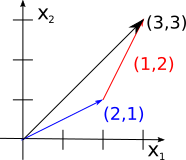
\includegraphics[width = 0.9\linewidth]{1.png}
\end{minipage}

\paragraph{Cross Product:} The \textbf{cross product} of two vectors, $\vec{u}$ and $\vec{v}$, returns a \textbf{vector} that is \textbf{perpendicular to both $\vec{u}$ and $\vec{v}$}, and its length is equal to the area of the parallelogram formed by $\vec{u}$ and $\vec{v}$

\color{theorem} \paragraph{Definition:} \textit{The Cross Product of two 3-dimensional vectors, $\vec{u} = \vect{u_1, u_2, u_3}$ and $\vec{v}=\vect{v_1,v_2,v_3}$}, is defined as the vector
\begin{equation}\label{eq:crossProduct}
\vec{u}\times\vec{v}= \vect{u_2\cdot v_3-u_3\cdot v_2\quad, u_3\cdot v_1-u_1\cdot v_3\quad, u_1\cdot v_2-u_2\cdot v_1}
\end{equation}
\color{black}  

\paragraph{Example:} Let's calculate the cross product of the vectors \color{groen} $\vec{u}=\vect{2,0,1}$ \color{black}and \color{rooj} $\vec{v}=\vect{2,1,-2}$ \color{black} using \ref{eq:crossProduct}

\begin{align*}
\color{groen} \vect{2,0,1} \color{black} \times \color{rooj} \vect{2,1,-2}\color{black} &= 
\icol{(0\cdot -2) - (1\cdot 1) \\ (1\cdot 2) - (2 \cdot -2) \\ (2 \cdot 2) - (0 \cdot 1)}
=\vect{-1,6,2}
\end{align*}

and the area of the parallelogram

\begin{align*}
|\vec{u}\times \vec{v}| &= |\vect{-1,6,2}|\\
&= \sqrt{(-1)^2+6^2+2^2}\\
&=\sqrt{41}
\end{align*}


\paragraph{Exercise:} Do the same for $\vec{u} = \vect{6,3,1}$ and $\vec{v} = \vect{0,2,5}$.


%Only 3d vectors



\end{document}